\section{Verificación y validación}

\frame{\sectionpage}

\begin{frame}{Verificación y validación}
    %\begin{itemize}
        %\item La verificación y la validación se ocupan de determinar si un modelo y sus resultados son 'correctos' para un uso o propósito específico.
        \begin{itemize}
            \item La \textit{verificación} se define como 'asegurar que el modelo programado y su implementación sean correctos'.
            \item La \textit{validación} se define como la 'comprobación de que el modelo de simulación dentro de su dominio de aplicabilidad posee un rango satisfactorio de precisión consistente con la aplicación prevista del modelo'.
        \end{itemize}
    %\end{itemize}    
\end{frame}

\begin{frame}{Proceso de desarrollo de modelos}
    \begin{figure}
        \centering
        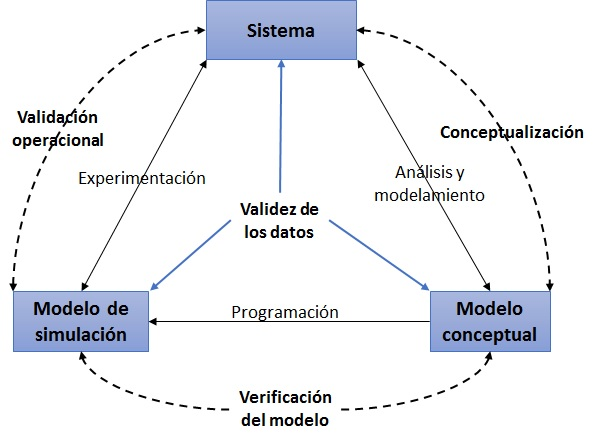
\includegraphics[width=9cm]{images/vandv.jpg}
        %\caption{Proceso de desarrollo de modelos}
        \label{fig:my_label4}
    \end{figure}
\end{frame}

\begin{frame}{Verificación}
    \begin{itemize}
        \item La verificación evalúa la exactitud de la representación formal del modelo previsto, a través de:
        \begin{enumerate}
            \item Depurador
            \item Animación
            \item Estadísticas básicas de las corridas de prueba
            \item Modelos de teoría de colas
        \end{enumerate}
    \end{itemize}
\end{frame}

\begin{frame}{Validación}
    \begin{itemize}
        \item La validación compara (estadísticamente) las medidas de desempeño del modelo, obtenidas en las corridas de prueba, con sus contrapartes en el sistema.
    \end{itemize}
\end{frame}

\begin{frame}{Validación - Ejemplo}
    \begin{itemize}
        \item Se tiene una muestra de demoras diarias en un cierto proceso del sistema real y la serie de datos de dichas demoras en el modelo simulado.
        \item Se podría definir una muestra de las diferencias observadas como \begin{equation*}
            G_i=\Hat{D_i}-\bar{D_i},~i=1,\dots, N
        \end{equation*}
        que sigue una distribución normalmente distribuida con media $\mu_G$ y varianza $\sigma^2_G$. Donde $\bar{D_i}$ es la media observada de la demora para el día $i$ en el sistema real y $\Hat{D_i}$ es la media estimada de la demora en el día $i$ tomada del modelo de simulación, para los días $i=1,\dots, N$.
    \end{itemize}
\end{frame}

\begin{frame}{Validación - Ejemplo}
    \begin{itemize}
        \item Se plantean las hipótesis 
        \begin{eqnarray*}
            H_0:~\mu_G=0\\
            H_1:~\mu_G \neq 0
        \end{eqnarray*}
        \item Bajo la hipótesis nula, el estadístico
        \begin{equation*}
            t_{N-1}=\frac{\bar{G}-\mu_G}{\frac{S_G}{\sqrt{N}}}
        \end{equation*}
        se distribuye de acuedo a un distribución $t$ de Student, con $N-1$ grados de libertad, donde $\bar{G}$ y $S_G$ son la media y desviación estándar de la muestra $\{G_1,\dots,G_N\}$, respectivamente.
    \end{itemize}
\end{frame}

\begin{frame}{Validación - Ejemplo}
    \begin{itemize}
        \item Para un nivel de significancia $\alpha$, el correspondiente intervalo de confianza es
        \begin{equation*}
            \bar{G}-t_{\frac{\alpha}{2},N-1}\frac{S_G}{\sqrt{N}}\leq \mu_G \leq \bar{G}+t_{\frac{\alpha}{2},N-1}\frac{S_G}{\sqrt{N}}
        \end{equation*}
        \item Si el intervalo de confianza anterior contiene 0, no se puede rechazar $H_0$ en el nivel de significancia $\alpha$, lo que indica que la prueba respalda la validez del modelo.
    \end{itemize}
\end{frame}